

\section{Why we need MRE}

% 
% \frame{\titlepage}

\begin{frame}[t]{Why do we need MRE?}

% \vspace{-\baselineskip}
% \begin{center}
% 	\define{Environmental monitoring problems} are of great \\ importance in many practical applications.
% \end{center}

% \vspace{.5\baselineskip}

\begin{columns}[T]
\column{.4\textwidth}
  \begin{itemize}
    \item<2-> diseased tissue changes mechanical
    \item<3-> low tech: palpation
    \item<4-> higher tech: ultrasound
    \item<5-> highest tech: MRE
    \item<6-> for deep tissue and brains, but non-invasive
  \end{itemize}
\column{.6\textwidth}

 	\vspace{-0.5cm}
	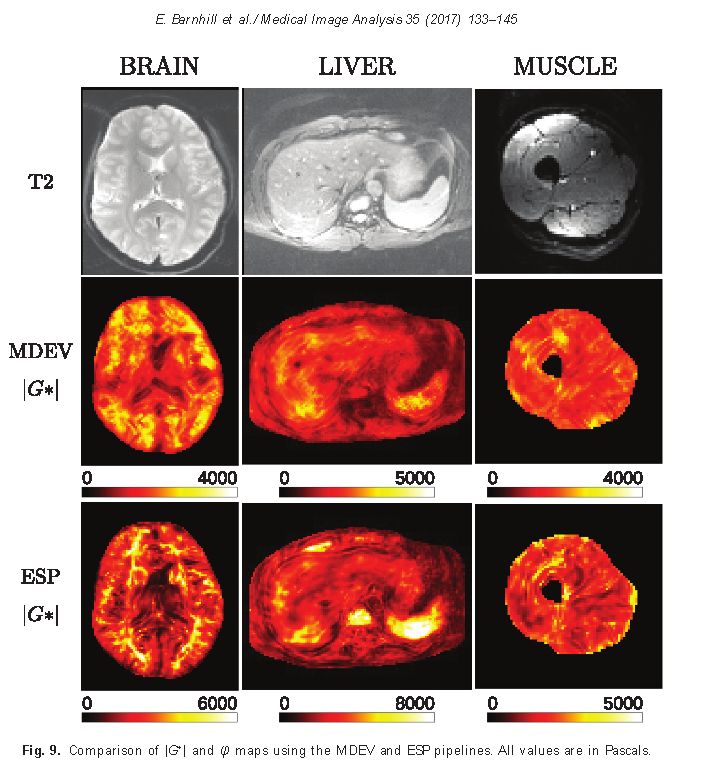
\includegraphics[width=\textwidth]{Images/Elasto-Tissue.pdf}

\end{columns}

\end{frame}



\begin{frame}{How does the measuring process work}

\begin{figure}
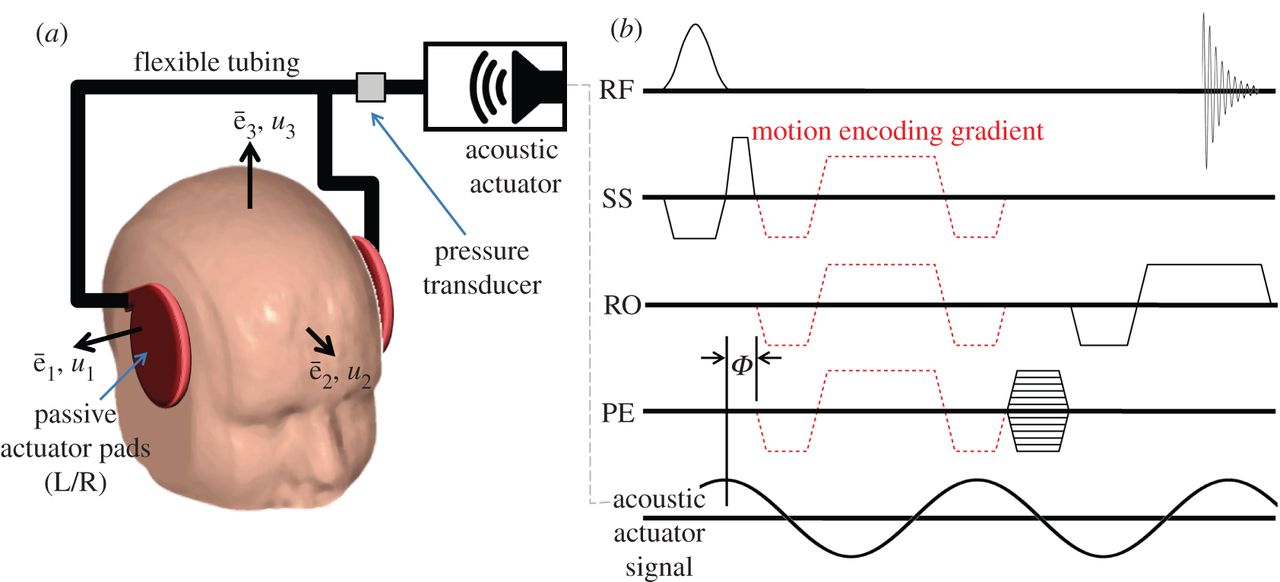
\includegraphics[width=0.9\textwidth]{Images/experiment.jpg}
\centering\end{figure}

\begin{itemize}
 \item<2-> 3 spatial directions $\times$ 8 time steps $\times$ 3 frequencies
 \item<3-> 72 times longer per pixel than MRI 
\end{itemize}

\end{frame}

\section{Data Reconstruction and current Problems}


\begin{frame}		\frametitle{Data reconstruction}


\begin{align}
 \mathbf{u} &= \mathbf{u}(\xb,t) \\
 \mu &=
\end{align}


\begin{equation}
 \sum_ j \partial_j \kl{ \mu \kl{ \partial_j u_i + \partial_i u_j}} + \partial_i \kl{\lambda \partial_j u_j} = \rho \ddot{u}_i
\end{equation}

\begin{equation}
 A\mathbf{\mu} = \mathbf{b}
\end{equation}


\end{frame}

\begin{frame}{Underdetermined System}


\begin{itemize}
 \item differential equation --> inverse problem
 \item Problem underdetermined, we need boundary values
 \item Problem: some regions are close to nodes --> no movement
 \item Solution: Multi frequency inversion
 \item Problem: Need to reconstruct the derivatives
 \item motion encoding gradient
 \item MRI measurement in 3 spatial directions and 8 time steps
\end{itemize}

\begin{itemize}
 \item MRI measurement in 3 spatial directions and 8 time steps and 3 frequencies --> 72 times MRI overhead
 \item --> reduced resolution
\end{itemize}

\begin{itemize}

 \item Problem: Need to reconstruct the derivatives
 \item slight noise can lead to totally wrong derivatives --> inversion is useless
 \item MRI measurement in 3 spatial directions and 8 time steps
\end{itemize}

\end{frame}

\section{Denoising Techniques}



\section{First Experiments}


\begin{frame}		\frametitle{Our plan of work}

\begin{itemize}
 \item Do simuations in 1d: wavelets
 \item Do simulations in 2d: wavelets, shearlets
 \item 
\end{itemize}

\begin{itemize}
 \item Problem: Need to reconstruct the derivatives
 \item slight noise can lead to totally wrong derivatives --> inversion is useless
 \item MRI measurement in 3 spatial directions and 8 time steps --> 
\end{itemize}

\end{frame}

\section{What comes next}


\begin{frame}		\frametitle{What would be nice results}

\begin{itemize}
 \item Have better resolution of the stiffness map
 \item Have clinically useful values, at the moment to varying
 \item Have shorter acquisition times per pixel
\end{itemize}

\begin{itemize}
 \item Problem: Need to reconstruct the derivatives
 \item slight noise can lead to totally wrong derivatives --> inversion is useless
 \item MRI measurement in 3 spatial directions and 8 time steps --> 
\end{itemize}

\end{frame}





 